\section{Equal-DOF baseline comparisons}
\label{sec:results}

\subsection{Comparison setup}

To assess approximation accuracy at matched coefficient counts, we compare five cases using a common evaluator: linear and cubic energies in one dimension, the sinh energy in two dimensions, and pure \(p=4\) energies in one and two dimensions, denoted C1--C5 in this order. The comparison counts retained CGA/RFM coefficients and independent FEM coefficients after removal of the constant mode where required.

For CGA, the comparison optimizes coefficients on fixed greedy prefixes. FEM uses uniform one-dimensional or structured triangular meshes with P1 and P3 references and supplementary P2 states. RFM uses nested normalized \(\relu^3\) features with ten prescribed seeds, 201--210, at each width. Supplement~S4 specifies the sampling, fitting, and evaluation protocol.

Figures join computed dyadic states and terminal CGA prefixes, while FEM curves use the mesh coefficient counts. The display ranges end at the corresponding CGA terminal widths. Table endpoints are \(256,256,256,128,256\) for C1--C5. FEM values use a computed state at the requested count when available and otherwise log--log interpolation between bracketing metric-valid states. The C3 P3 value is computed directly at \(N=256\).

\subsection{Evaluation and statistical samples}

An observation enters a metric summary when the solve succeeds, the metric is finite and nonnegative, and successive evaluation quadratures have a relative difference of at most one percent. The same rule applies to all methods. Energy differences retain their sign in the numerical records. Each of the energy, Sobolev, and \(V\)-distance summaries uses its own valid observations.

RFM medians and interquartile ranges are computed from the valid observations for each metric. In \Cref{tab:baseline-terminal}, \emph{Valid} gives the number of valid Sobolev observations out of the ten prescribed seeds. Supplement~S3 lists the solve statuses, metric sample counts, and model identifiers.

\subsection{Relative Sobolev errors}

C1--C3 report relative \(H^1\) errors, and C4--C5 report the relative componentwise gradient \(L^4\) seminorm \(e_{\nabla,4}\) defined in \Cref{sec:numerics}. The \(V\)-distance is reported in the following subsection.

\begin{figure}[!htbp]
\centering
\subfloat[Linear, \(d=1\).]{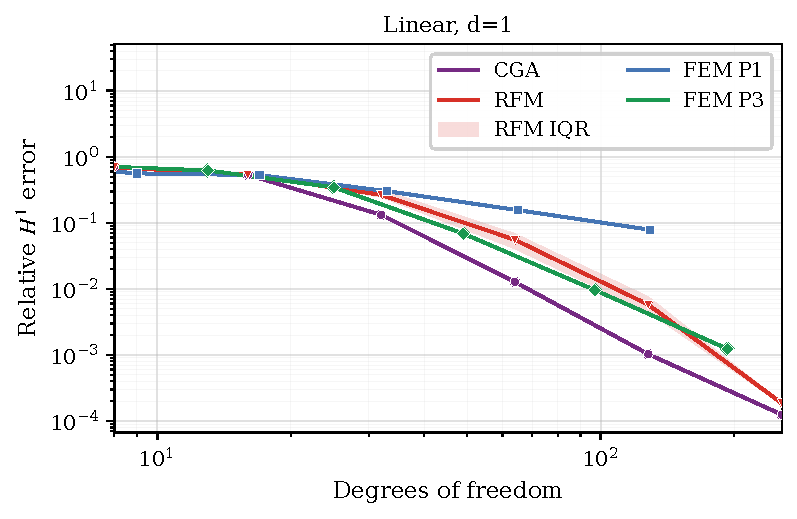
\includegraphics[width=0.49\textwidth]{C1_relative_h1_error.pdf}}\hfill
\subfloat[Cubic, \(d=1\).]{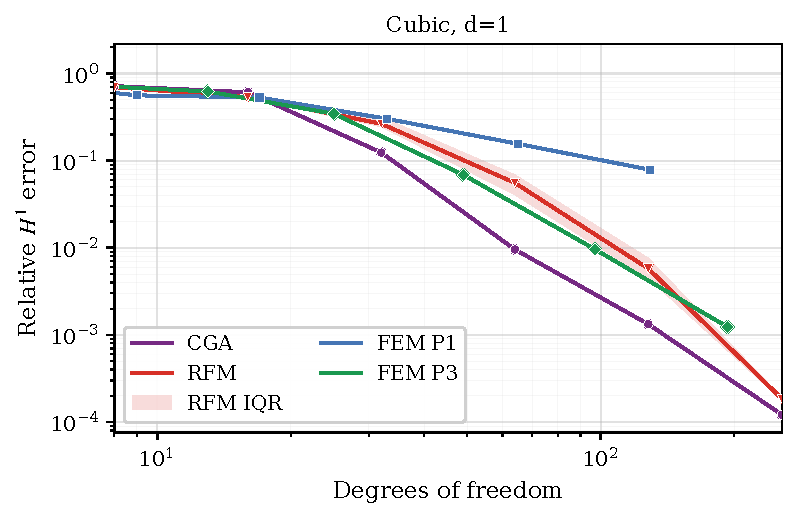
\includegraphics[width=0.49\textwidth]{C2_relative_h1_error.pdf}}
\caption{Relative \(H^1\) error versus coefficient count for the
one-dimensional comparison. RFM bands show metric-valid medians and
interquartile ranges from ten prescribed seeds. Markers are computed states;
CGA coefficients are refitted on fixed greedy prefixes.}
\label{fig:baseline-sobolev-1d}
\end{figure}

\begin{figure}[!htbp]
\centering
\subfloat[Sinh, \(d=2\): \(H^1\).]{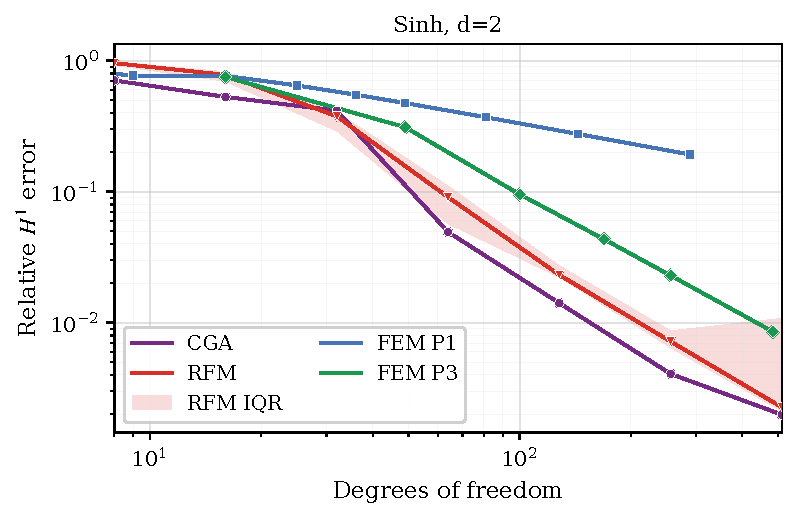
\includegraphics[width=0.32\textwidth]{C3_relative_h1_error.pdf}}\hfill
\subfloat[Pure \(p=4,d=1\): \(e_{\nabla,4}\).]{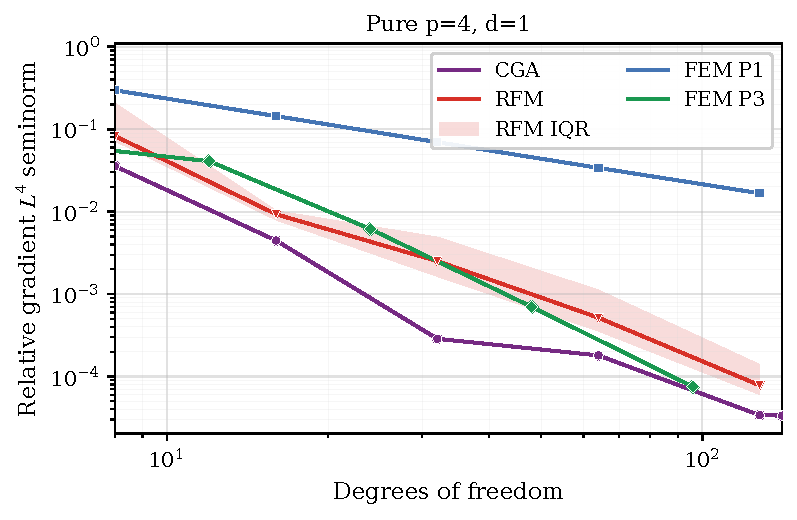
\includegraphics[width=0.32\textwidth]{C4_relative_w1p_error.pdf}}\hfill
\subfloat[Pure \(p=4,d=2\): \(e_{\nabla,4}\).]{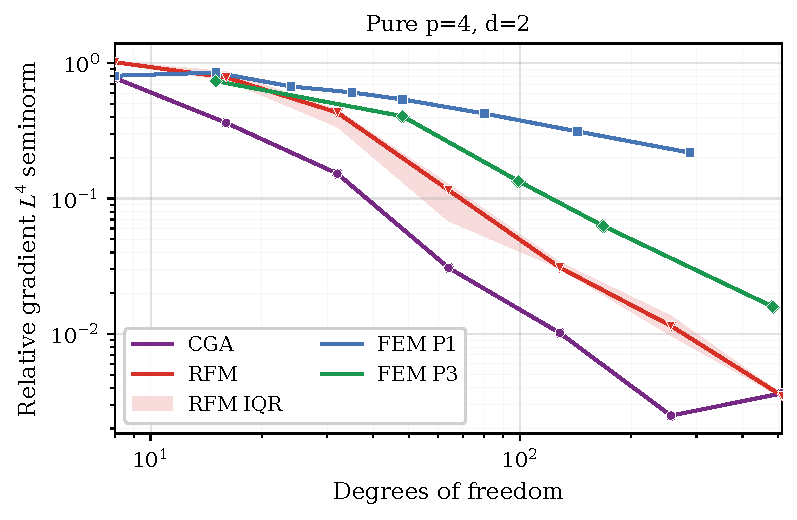
\includegraphics[width=0.32\textwidth]{C5_relative_w1p_error.pdf}}
\caption{Relative \(H^1\) error for sinh and relative gradient
\(L^4\) seminorm for the pure \(p=4\) problems. RFM bands summarize the
metric-valid observations from ten prescribed seeds. Endpoint valid counts
appear in \Cref{tab:baseline-terminal}.}
\label{fig:baseline-sobolev-rest}
\end{figure}
\FloatBarrier

\Cref{tab:baseline-terminal} reports the endpoint errors and comparator-to-CGA ratios. A ratio above one indicates a smaller CGA error. CGA has smaller errors than the metric-valid RFM medians at all five endpoints and smaller errors than the P3 FEM references in four cases. For the one-dimensional pure \(p=4\) case at \(N=128\), the P3/CGA and RFM-median/CGA ratios are approximately 0.88 and 2.30, respectively.
\begin{table}[!htbp]
\centering\scriptsize
\caption{Endpoint relative \(H^1\) errors for C1--C3 and relative gradient \(L^4\) seminorm errors for C4--C5. RFM values are median [Q1,Q3] over metric-valid observations from ten prescribed seeds. Valid gives the Sobolev sample count; the inclusion rule is defined in the text. The P3 value for C3 is computed directly, and the other P3 endpoint values use log--log interpolation between bracketing metric-valid states. Ratios above one indicate smaller CGA errors.}
\label{tab:baseline-terminal}
\resizebox{\linewidth}{!}{%
\begin{tabular}{@{}crrrrrr@{}}
\toprule
Problem & DOF & CGA & RFM median [Q1,Q3] & Valid & RFM/CGA & FEM P3/CGA \\ \midrule
Linear, d=1 & 256 & $1.247\!\times\!10^{-4}$ & $1.853\!\times\!10^{-4}$ [$1.779\!\times\!10^{-4}$, $1.913\!\times\!10^{-4}$] & 10/10 & 1.49 & 4.24 \\
Cubic, d=1 & 256 & $1.215\!\times\!10^{-4}$ & $1.853\!\times\!10^{-4}$ [$1.779\!\times\!10^{-4}$, $1.913\!\times\!10^{-4}$] & 10/10 & 1.52 & 4.35 \\
Sinh, d=2 & 256 & $4.074\!\times\!10^{-3}$ & $7.196\!\times\!10^{-3}$ [$6.472\!\times\!10^{-3}$, $8.663\!\times\!10^{-3}$] & 10/10 & 1.77 & 5.63 \\
Pure p=4, d=1 & 128 & $3.395\!\times\!10^{-5}$ & $7.818\!\times\!10^{-5}$ [$6.046\!\times\!10^{-5}$, $1.400\!\times\!10^{-4}$] & 10/10 & 2.30 & 0.88 \\
Pure p=4, d=2 & 256 & $2.493\!\times\!10^{-3}$ & $1.147\!\times\!10^{-2}$ [$9.730\!\times\!10^{-3}$, $1.360\!\times\!10^{-2}$] & 6/10 & 4.60 & 14.54 \\
\bottomrule
\end{tabular}}
\end{table}

\FloatBarrier

\subsection{Natural \texorpdfstring{\(V\)}{V}-distance for the \texorpdfstring{\(p\)}{p}-models}

\Cref{fig:baseline-v} reports the relative \(V\)-distance for the pure \(p=4\) models. Each curve uses computed states, and the RFM bands show the median and interquartile range of the observations valid for this metric.

\begin{figure}[!htbp]
\centering
\subfloat[Pure \(p=4,d=1\).]{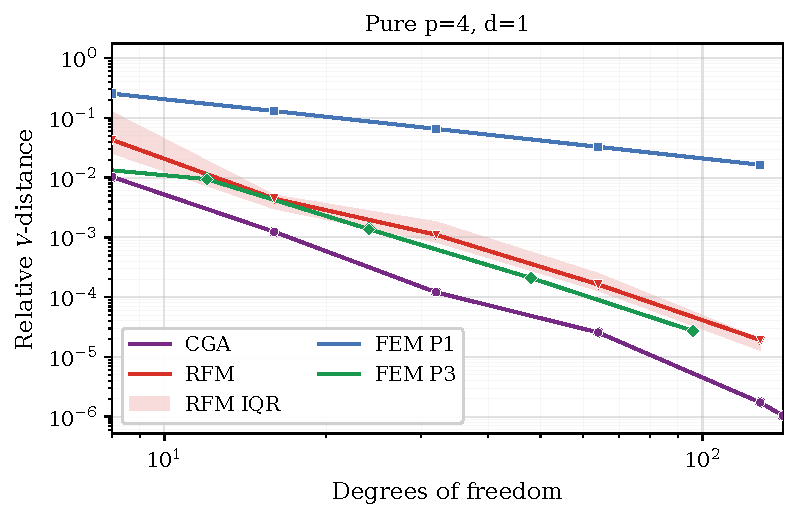
\includegraphics[width=0.49\textwidth]{C4_v_distance.pdf}}\hfill
\subfloat[Pure \(p=4,d=2\).]{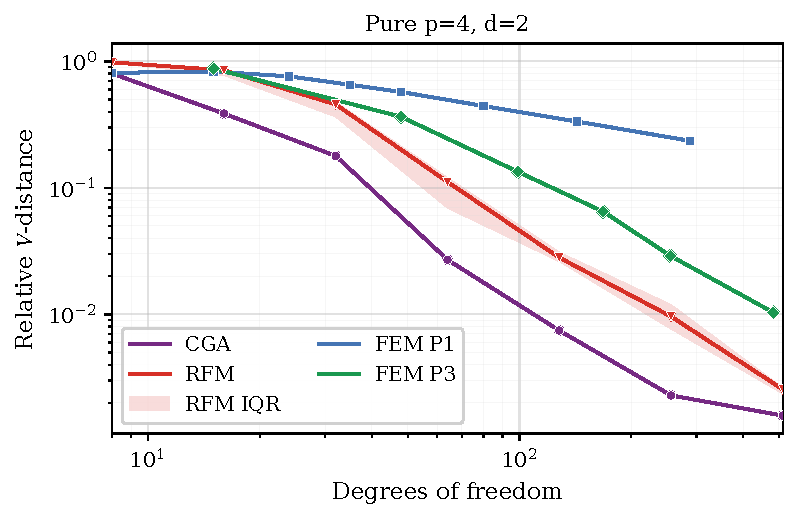
\includegraphics[width=0.49\textwidth]{C5_v_distance.pdf}}
\caption{Relative \(V\)-distance versus coefficient count for the pure \(p=4\) comparisons. Markers show computed states; RFM bands show metric-valid medians and interquartile ranges.}
\label{fig:baseline-v}
\end{figure}
\FloatBarrier
